\subsection{NEON}
\subsubsection{Function Analysis}

The nature of Gaussian blur is to convolve the image with Gaussian function. In the original program, the Gaussian filter, which is called kernel in the application, has fifteen Gaussian values to blur a single pixel. This implementation illustrates that seven neighbor values on both sides of a pixel, and the value of the pixel itself are taken to do the calculation. In C code, the calculation is executed by using for-loop iteration for each value. While in the NEON implementation, we decided to take the advantage of parallel computing of NEON; calculating multiple values at the same time.

\subsubsection{Implementation}

In \textit{gaussian\_smooth} function, the blurred value are stored in single-precision floating-point. For NEON, four same operations based on single-precision floating-point can be performed simultaneously. Since the number of Gaussian values is not a multiple of four, we decided to have some modifications to implement the operation on NEON. 

Originally, seven neighbor values are taken on either side of a pixel. In our case, we decided to take values from eight neighbors (two times of NEON calculation)for calculating simplicity. However, in order to coincide with the original calculation, the corresponding Gaussian value of newly added neighbors are set to zero to ensure they do not affect the calculation output at the end. In the implementation, we take an extra value at both the left-most side and right-most side of the neighbor, and adding two extra zeros at both the head and tail of the Gaussian filter. Figure~\ref{fig:newfilter} shows how the Gaussian kernel is modified and split for NEON implementation. Different from other Gaussian values, kernel[8] is used separately for the calculation of the pixel itself. 

\begin{figure*}
\centering
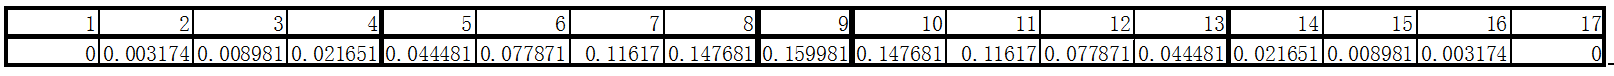
\includegraphics[width=\linewidth]{drawings/filter}
\caption{Modified filter}
\label{fig:newfilter}
\end{figure*}

We also had modifications for the blurring of pixels located near the boundary. For example, the pixel located on the left-most side does not have left neighbors for Gaussian blur. In the sequential implementation, the boundary check is performed by if-statement conditional checking. In our implementation, instead of boundary check, we add eight more cols (filled with zeros) on either the left or right most side of the image to ensure every pixel has 8 neighbors on both sides. Figure~\ref{fig:addcols} illustrates how the new image is stored for NEON calculation. 

\begin{figure}
\centering
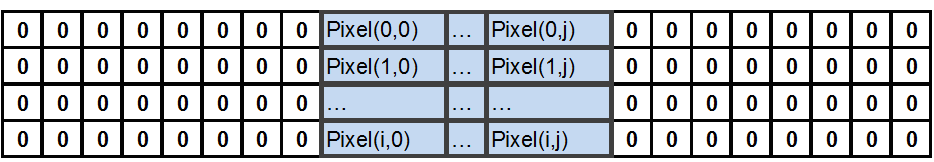
\includegraphics[width=0.4\textwidth]{drawings/new_cols}
\caption{Modified image for NEON implementation}
\label{fig:addcols}
\end{figure}

As a result, Figure~\ref{fig:neon} represents how the total product value of Gaussian smooth is performed for each pixel. The calculations based on neighbor values are performed four times, during each time, four neighbor values are calculated concurrently. To obtain the final product value, values from each lane and blurred value based on the current pixel are summed up at the end.

\begin{figure*}
\centering
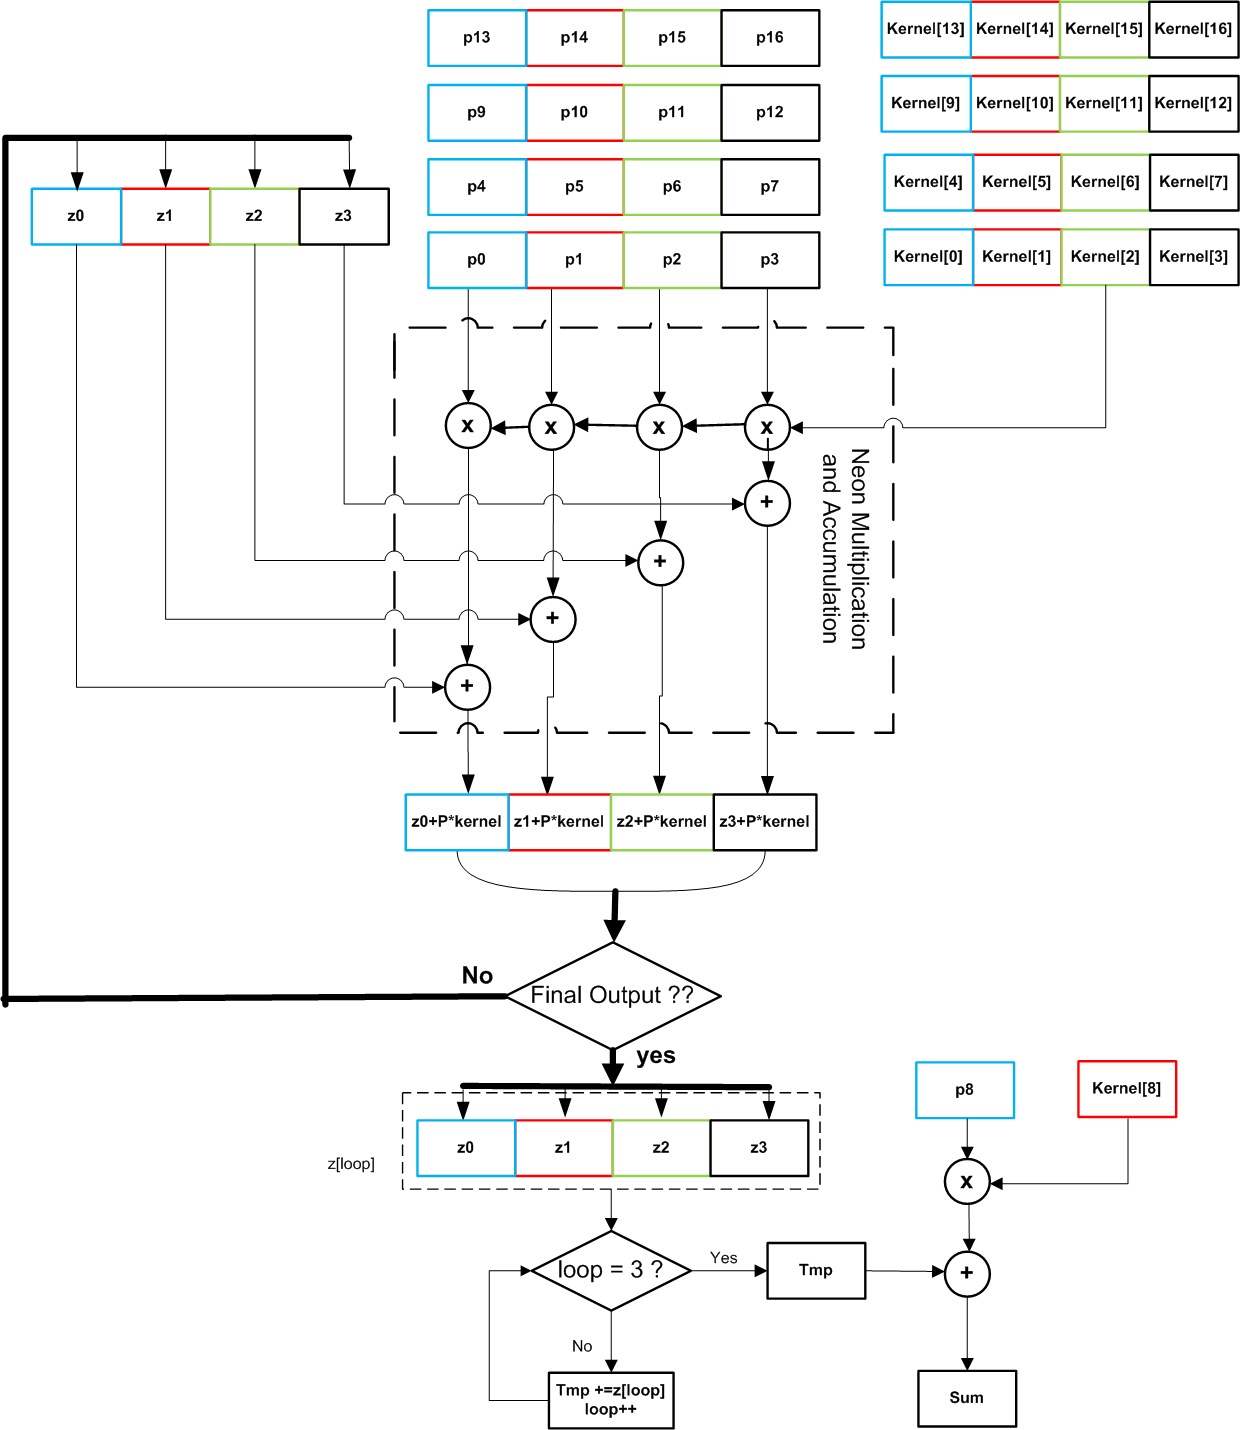
\includegraphics[width=0.6\linewidth]{drawings/neon}
\caption{NEON implementation of Gaussian smooth}
\label{fig:neon}
\end{figure*}
